\documentclass{BeamerTemplate}

\title{Chapitre 2 -- La théorie des probabilités (2\textsuperscript{e} partie)}
\subtitle{STT-1920 Méthodes statistiques}
\date{}

% Code R et sortie console
\DefineVerbatimEnvironment{console}{Verbatim}{fontsize=\scriptsize, formatcom=\color{TexteBoite}}

% Styles des graphiques
\pgfplotsset{
  base/.style={
    tick label style={font=\scriptsize}, label style={font=\small},
    title style={font=\small\bfseries},
    yticklabel style={/pgf/number format/fixed, /pgf/number format/precision=2},
    scaled y ticks=false,
  },
  petit/.style={base, width=0.49\textwidth, height=0.42\textheight, ymin=0,
    tick label style={font=\tiny}, label style={font=\scriptsize},
    title style={font=\scriptsize\bfseries, yshift=-4pt}},
  batons/.style={ycomb, thick, color=Accent, mark=*, mark size=1pt, mark options={fill=Accent}},
}

\begin{document}

\begin{frame}[t]
  \titlepage
\end{frame}

%===============================================================================
\section{Introduction}
%===============================================================================

\begin{frame}[t]{Contexte}
  Il existe plusieurs lois de probabilité bien connues, qui ont même un
  \alert{nom}, et pour lesquelles on connaît bien le comportement et les
  caractéristiques (espérance, variance, forme).

  \medskip
  Plusieurs de ces lois sont reliées à des expériences aléatoires simples, par
  exemple une expérience qui résulte en un \alert{succès} ou un \alert{échec}.

  \medskip
  \uncover<2->{
  \begin{Boite}{Épreuve de Bernoulli}
    Expérience aléatoire ayant deux résultats possibles que l'on désigne
    arbitrairement par SUCCÈS et ÉCHEC. On note $p$ la probabilité de succès.
  \end{Boite}
  }
  \uncover<3->{
  {\small
  Exemples : le sexe d'un nouveau-né (mâle / femelle); l'état d'un arbre (mort
  / vivant); une tumeur (bénigne / maligne); la germination d'une graine
  (oui / non).}
  }
\end{frame}

\begin{frame}[t]{Quelques lois classiques}
  \scriptsize
  \renewcommand{\arraystretch}{1.25}
  \begin{tabularx}{\textwidth}{@{}l X@{}}
    \toprule
    \textbf{Loi (section des notes)} & \textbf{Contexte typique} \\
    \midrule
    \alert{Binomiale} (2.6.1) & Nombre de succès parmi $n$ épreuves de Bernoulli indépendantes \\
    Géométrique (2.6.2) & Nombre d'épreuves de Bernoulli indépendantes pour obtenir un succès \\
    Hypergéométrique (2.6.3) & Nombre de succès parmi $n$ épreuves (tirages sans remise) \\
    \alert{Poisson} (2.6.4) & Nombre d'événements dans un intervalle de temps (ou d'espace) \\
    Uniforme continue (2.6.5) & Densité constante sur $[a, b]$ \\
    \alert{Normale} (2.6.6) & Plusieurs phénomènes; loi d'une somme ou d'une moyenne (TLC) \\
    Student (3.5.2) & Moyenne d'un échantillon normal de variance inconnue \\
    $\chi^2$ (3.6.2) & Variance d'un échantillon normal; tableaux de fréquences \\
    Fisher (4.2.2) & Comparer des variances \\
    \bottomrule
  \end{tabularx}

  \medskip
  Dans ce chapitre : les lois \alert{binomiale}, de \alert{Poisson} et \alert{normale}.
\end{frame}

\begin{frame}[t]{Un concept important : v.a.\ indépendantes}
  Dans ce chapitre, on parlera souvent de variables aléatoires indépendantes.

  \begin{Boite}{Variables aléatoires indépendantes}
    Deux variables aléatoires sont \alert{indépendantes} si connaître la valeur
    de l'une ne nous renseigne en rien sur la valeur de l'autre.
  \end{Boite}

  \uncover<2->{
  Rappel (chapitre 2, 1\textsuperscript{re} partie) : si $X$ et $Y$ sont
  indépendantes,
  \[ \operatorname{Var}(X + Y) = \operatorname{Var}(X) + \operatorname{Var}(Y). \]
  }
  \uncover<3->{
  \textbf{Exemple :} je note le sexe d'un veau ($X = 1$ si femelle) et je lance
  un dé ($Y$ = face obtenue). $X$ et $Y$ sont indépendantes.
  }
\end{frame}

%===============================================================================
\section[Loi binomiale]{2.6.1 La loi binomiale}
%===============================================================================

\begin{frame}[t]{Loi de Bernoulli}
  Soit $Y$ une variable aléatoire telle que $Y = 1$ si l'épreuve est un succès
  et $Y = 0$ si c'est un échec.

  \begin{defn}
    On dit que $Y$ suit une \alert{loi de Bernoulli} de paramètre $p$, noté
    $Y \sim \text{Bernoulli}(p)$, si
    \[
      p(y) =
      \begin{cases}
        p & \text{si } y = 1, \\
        1 - p & \text{si } y = 0, \\
        0 & \text{sinon.}
      \end{cases}
    \]
  \end{defn}

  Espérance : \hspace{5cm} Variance :
\end{frame}

\begin{frame}[t]{Exemple 1}
  Selon la directive européenne pour la commercialisation des semences de
  céréales, le taux de germination minimal pour les grains d'avoine doit être
  de 85\,\%. Vous plantez 5 grains d'un lot qui suit cette norme.

  \medskip
  \alert{Quelle est la probabilité qu'un seul grain ne germe pas?}

  \medskip
  \uncover<2->{
  \begin{itemize}\itemsep 2mm
    \item Épreuve de Bernoulli : planter un grain; succès = il germe.
    \item Probabilité de succès : $p = 0.85$.
    \item Nombre d'épreuves (indépendantes) : $n = 5$.
  \end{itemize}
  }
  \uncover<3->{
  Résultats avec exactement un échec ($E$) :
  \[ EGGGG, \quad GEGGG, \quad GGEGG, \quad GGGEG, \quad GGGGE \]
  Chacun a probabilité $0.85^4 \times 0.15$\ldots\ et il y en a combien?
  }
\end{frame}

\begin{frame}[t]{Rappel : coefficient binomial (section 2.3.4)}
  \begin{Boite}{Coefficient binomial}
    Le nombre de sous-ensembles de $r$ objets choisis sans remise parmi $n$
    objets distincts est
    \[ \binom{n}{r} = \frac{n!}{r!\,(n-r)!}. \]
  \end{Boite}

  \begin{itemize}\itemsep 1.6cm
    \item Combien de sous-ensembles de 2 éléments peut-on former à partir de
      l'ensemble $\{A, B, C, D, E\}$?
    \item Combien d'échantillons différents de taille 6 peut-on tirer d'une
      population de taille 49?
  \end{itemize}
\end{frame}

\begin{frame}[t]{Loi binomiale}
  Soit $Y_1, \ldots, Y_n$ des v.a.\ \alert{indépendantes} de loi
  Bernoulli($p$), et $X = Y_1 + Y_2 + \cdots + Y_n$ le nombre total de succès.
  \medskip

  \uncover<2->{
  {\small On cherche la probabilité d'avoir $k$ succès, donc $n - k$ échecs.}
  \begin{itemize}\small
    \item Chaque résultat avec $k$ succès a probabilité $p^k (1-p)^{n-k}$.
    \item Il y a $\binom{n}{k}$ façons de placer les $k$ succès parmi les $n$ épreuves.
  \end{itemize}
  }
  \uncover<3->{
  \begin{defn}
    $X$ suit une \alert{loi binomiale} de paramètres $n$ et $p$, noté
    $X \sim \text{Binomiale}(n, p)$ :
    \[
      p(k) = P(X = k) =
      \begin{cases}
        \dbinom{n}{k} p^k (1-p)^{n-k} & \text{si } k \in \{0, 1, \ldots, n\}, \\[2mm]
        0 & \text{sinon.}
      \end{cases}
    \]
  \end{defn}
  }
\end{frame}

\begin{frame}[t]{Allure de la loi binomiale}
  \centering
  \begin{tikzpicture}
    \begin{axis}[petit, title={Binomiale(10, 0.2)}, xlabel={$x$}, ylabel={$p(x)$}]
      \addplot[batons] coordinates {(0,0.10737) (1,0.26844) (2,0.30199) (3,0.20133) (4,0.08808) (5,0.02642) (6,0.00551) (7,0.00079) (8,0.00007) (9,0.00000) (10,0.00000)};
    \end{axis}
  \end{tikzpicture}\hfill
  \begin{tikzpicture}
    \begin{axis}[petit, title={Binomiale(10, 0.5)}, xlabel={$x$}, ylabel={$p(x)$}]
      \addplot[batons] coordinates {(0,0.00098) (1,0.00977) (2,0.04395) (3,0.11719) (4,0.20508) (5,0.24609) (6,0.20508) (7,0.11719) (8,0.04395) (9,0.00977) (10,0.00098)};
    \end{axis}
  \end{tikzpicture}

  \raggedright\small
  Dans tous les cas :
  \begin{itemize}
    \item les valeurs possibles sont $0, 1, 2, \ldots, n$;
    \item les valeurs les plus probables sont autour de $np$;
    \item la fonction de masse croît jusqu'à environ $np$, puis décroît.
  \end{itemize}
\end{frame}

\begin{frame}[t]{Espérance et variance}
  \begin{prp}
    Si $X \sim \text{Binomiale}(n, p)$, alors
    \[ \mu = E(X) = np \qquad \text{et} \qquad \sigma^2 = \operatorname{Var}(X) = np(1-p). \]
  \end{prp}

  \uncover<2->{
  Pourquoi? On écrit $X = Y_1 + \cdots + Y_n$ avec $Y_i \sim \text{Bernoulli}(p)$
  indépendantes :
  \begin{align*}
    E(X) &= E(Y_1) + \cdots + E(Y_n) = p + \cdots + p = np, \\
    \operatorname{Var}(X) &= \operatorname{Var}(Y_1) + \cdots + \operatorname{Var}(Y_n) = np(1-p).
  \end{align*}
  {\small\color{gray}[propriétés 2 et 4 de l'espérance et de la variance, 1\textsuperscript{re} partie]}
  }
\end{frame}

\begin{frame}[t]{Exemple 1 (suite)}
  Vous plantez 5 grains d'un lot dont le taux de germination est de 85\,\%.

  \medskip
  \alert{Quelle est la probabilité qu'un seul grain ne germe pas?}
\end{frame}

\begin{frame}[t]{Exemple 2}
  Une étude révèle que 95\,\% des canards colverts ont des parasites internes.
  Un biologiste capture 7 canards lors d'une séance d'échantillonnage.

  \begin{enumerate}[a)]\itemsep 1.4cm
    \item Quelle est la probabilité qu'il capture plus de 5 canards infestés?
    \item Si plusieurs biologistes capturent 7 canards chacun, le nombre moyen
      de canards infestés devrait être environ\ldots
    \item L'écart type du nombre de canards infestés par biologiste devrait
      valoir\ldots
  \end{enumerate}
\end{frame}

\begin{frame}[fragile,t]{Calculs dans R}
  Pour $X \sim \text{Binomiale}(n, p)$ :
  \texttt{dbinom(k, n, p)} donne $P(X = k)$ et \texttt{pbinom(k, n, p)} donne
  $P(X \le k)$.

  \medskip
  Exemple 1 : $P(\text{4 grains germent sur 5})$
\begin{console}
> dbinom(4, size = 5, prob = 0.85)
[1] 0.3915047
\end{console}

  Exemple 2 : $P(X > 5) = 1 - P(X \le 5)$
\begin{console}
> 1 - pbinom(5, size = 7, prob = 0.95)
[1] 0.9556195
\end{console}
\end{frame}

\begin{frame}[plain,t]
  \centerline{\LARGE\bfseries\alert{QUIZ !}}

  \medskip
  Deux parents sont porteurs sains (génotype $Aa$) de l'allèle récessif
  responsable de la fibrose kystique. Chacun de leurs enfants a une
  probabilité $1/4$ d'être atteint (génotype $aa$), indépendamment des autres.
  Le couple a 4 enfants; soit $X$ le nombre d'enfants atteints.
  \begin{itemize}\itemsep 1.2cm
    \item Quelle est la loi de $X$? Vérifiez les conditions.
    \item Combien d'enfants atteints ce type de famille a-t-il en moyenne?
    \item Quelle est la probabilité qu'aucun des 4 enfants ne soit atteint?
  \end{itemize}
\end{frame}

%===============================================================================
\section[Loi de Poisson]{2.6.4 La loi de Poisson}
%===============================================================================

\begin{frame}[t]{Contexte}
  La loi de Poisson sert à modéliser une \alert{fréquence} : un nombre
  d'événements qui se produisent pendant un certain temps ou dans un certain
  espace.

  \medskip
  Exemples :
  \begin{itemize}\small
    \item $X$ = nombre d'animaux qui s'abreuvent à une source en 1\,h;
    \item $Y$ = nombre de décès dus à la tuberculose en un mois;
    \item $Z$ = nombre de chevreuils par km$^2$ dans un parc national;
    \item $W$ = nombre de colonies de bactéries sur une plaque de gélose.
  \end{itemize}

  \uncover<2->{
  On l'obtient aussi comme \alert{loi des événements rares} : une binomiale
  avec $n$ très grand et $p$ très petit (on y revient plus loin).
  }
\end{frame}

\begin{frame}[t]{Conditions d'application}
  Pour que la loi de Poisson soit un bon modèle, il faut que la réalité
  s'approche des conditions suivantes :
  \begin{itemize}\itemsep 3mm
    \item les nombres d'événements dans des intervalles qui ne se chevauchent
      pas sont des v.a.\ \alert{indépendantes};
    \item les événements se produisent au hasard, mais à un \alert{taux moyen
      constant} sur tout l'intervalle considéré;
    \item la probabilité que deux événements ou plus surviennent
      \alert{simultanément} est nulle.
  \end{itemize}
\end{frame}

\begin{frame}[t]{Loi de Poisson}
  La loi de Poisson est caractérisée par un paramètre $\lambda$, le taux
  d'occurrence (nombre moyen d'événements) sur l'intervalle considéré.

  \begin{defn}
    $X$ suit une \alert{loi de Poisson} de paramètre $\lambda > 0$, noté
    $X \sim \text{Poisson}(\lambda)$, si
    \[
      p(k) = P(X = k) =
      \begin{cases}
        \dfrac{e^{-\lambda} \lambda^k}{k!} & \text{si } k \in \{0, 1, 2, \ldots\}, \\[3mm]
        0 & \text{sinon.}
      \end{cases}
    \]
  \end{defn}

  \uncover<2->{
  \begin{prp}
    Si $X \sim \text{Poisson}(\lambda)$, alors $E(X) = \lambda$ et
    $\operatorname{Var}(X) = \lambda$.
  \end{prp}
  }
\end{frame}

\begin{frame}[t]{Allure de la loi de Poisson}
  \centering
  \begin{tikzpicture}
    \begin{axis}[petit, title={Poisson(2)}, xlabel={$x$}, ylabel={$p(x)$}]
      \addplot[batons] coordinates {(0,0.13534) (1,0.27067) (2,0.27067) (3,0.18045) (4,0.09022) (5,0.03609) (6,0.01203) (7,0.00344) (8,0.00086) (9,0.00019) (10,0.00004) (11,0.00001) (12,0.00000) (13,0.00000) (14,0.00000) (15,0.00000) (16,0.00000) (17,0.00000) (18,0.00000) (19,0.00000) (20,0.00000)};
    \end{axis}
  \end{tikzpicture}\hfill
  \begin{tikzpicture}
    \begin{axis}[petit, title={Poisson(10)}, xlabel={$x$}, ylabel={$p(x)$}]
      \addplot[batons] coordinates {(0,0.00005) (1,0.00045) (2,0.00227) (3,0.00757) (4,0.01892) (5,0.03783) (6,0.06306) (7,0.09008) (8,0.11260) (9,0.12511) (10,0.12511) (11,0.11374) (12,0.09478) (13,0.07291) (14,0.05208) (15,0.03472) (16,0.02170) (17,0.01276) (18,0.00709) (19,0.00373) (20,0.00187)};
    \end{axis}
  \end{tikzpicture}

  \raggedright\small
  \begin{itemize}
    \item Les valeurs possibles sont tous les entiers non négatifs $0, 1, 2, \ldots$
    \item Les valeurs les plus probables sont concentrées autour de l'espérance $\lambda$.
    \item Plus $\lambda$ est grand, plus la distribution est étalée (car
      $\operatorname{Var}(X) = \lambda$) et symétrique.
  \end{itemize}
\end{frame}

\begin{frame}[t]{Siméon-Denis Poisson (1781--1840)}
  \begin{columns}[T]
    \column{0.5\textwidth}
      Le chirurgien manqué\ldots\ mais excellent mathématicien et physicien.
    \column{0.45\textwidth}
      \centering
      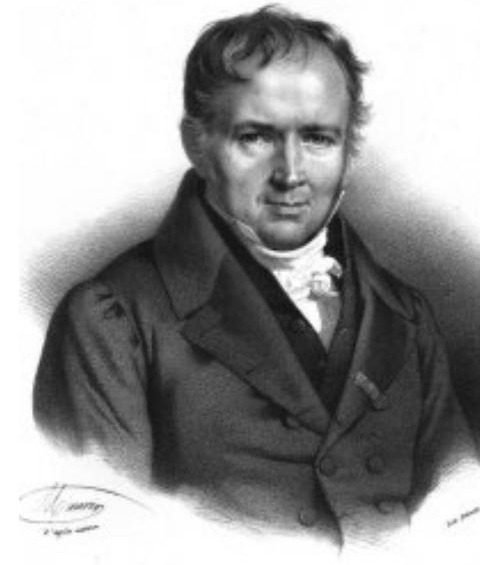
\includegraphics[height=0.72\textheight]{images/poisson.jpg}
  \end{columns}
\end{frame}

\begin{frame}[t]{Propriété d'additivité}
  \begin{prp}
    Si $X_1, \ldots, X_n$ sont des v.a.\ indépendantes avec
    $X_i \sim \text{Poisson}(\lambda_i)$, alors
    \[ X_1 + \cdots + X_n \sim \text{Poisson}(\lambda_1 + \cdots + \lambda_n). \]
  \end{prp}

  \uncover<2->{
  En pratique : si on observe en moyenne $\lambda$ événements par unité de
  temps (ou d'espace), le nombre d'événements dans $t$ unités suit une loi
  Poisson($\lambda t$).
  }
\end{frame}

\begin{frame}[t]{Exemple 3}
  Vous dénombrez les globules blancs sur une lame quadrillée présentant 25
  carrés de 0,1\,\si{\micro\liter} chacun. Supposons qu'il y a en moyenne 5
  globules blancs par carré.

  \begin{enumerate}[a)]\itemsep 2cm
    \item Quelle est la probabilité d'observer moins de 3 globules blancs sur
      un carré?
    \item Quelle est la probabilité d'observer 45 globules blancs dans un
      microlitre?
  \end{enumerate}
\end{frame}

\begin{frame}[fragile,t]{Calculs dans R}
  Pour $X \sim \text{Poisson}(\lambda)$ : \texttt{dpois(k, lambda)} donne
  $P(X = k)$ et \texttt{ppois(k, lambda)} donne $P(X \le k)$.

  \medskip
  Exemple 3 a) : $P(X < 3) = P(X \le 2)$ avec $\lambda = 5$
\begin{console}
> ppois(2, lambda = 5)
[1] 0.1246520
\end{console}

  Exemple 3 b) : un microlitre = 10 carrés, donc $\lambda = 10 \times 5 = 50$
\begin{console}
> dpois(45, lambda = 50)
[1] 0.04582624
\end{console}
\end{frame}

\begin{frame}[t]{Loi des événements rares}
  La loi de Poisson peut servir d'approximation de la loi binomiale lorsque
  $n$ est grand et $p$ petit, avec $\lambda = np$ :

  \medskip
  \centering
  \pgfplotsset{comp/.style={petit, height=0.6\textheight, ybar, bar width=0.3,
      xtick={0,...,12}, xlabel={$x$}, ylabel={Probabilité}, xmin=-0.7, xmax=12.7,
      legend style={font=\tiny, draw=none, fill=none}, legend cell align=left}}
  \begin{tikzpicture}
    \begin{axis}[comp, title={Binomiale(20, 0.2) et Poisson(4)}]
      \addplot[fill=Dominante, draw=none] coordinates {(0,0.01153) (1,0.05765) (2,0.13691) (3,0.20536) (4,0.21820) (5,0.17456) (6,0.10910) (7,0.05455) (8,0.02216) (9,0.00739) (10,0.00203) (11,0.00046) (12,0.00009)};
      \addplot[fill=Accent, draw=none] coordinates {(0,0.01832) (1,0.07326) (2,0.14653) (3,0.19537) (4,0.19537) (5,0.15629) (6,0.10420) (7,0.05954) (8,0.02977) (9,0.01323) (10,0.00529) (11,0.00192) (12,0.00064)};
      \legend{Binomiale, Poisson}
    \end{axis}
  \end{tikzpicture}\hfill
  \begin{tikzpicture}
    \begin{axis}[comp, title={Binomiale(200, 0.02) et Poisson(4)}]
      \addplot[fill=Dominante, draw=none] coordinates {(0,0.01759) (1,0.07179) (2,0.14577) (3,0.19635) (4,0.19735) (5,0.15788) (6,0.10472) (7,0.05923) (8,0.02916) (9,0.01270) (10,0.00495) (11,0.00174) (12,0.00056)};
      \addplot[fill=Accent, draw=none] coordinates {(0,0.01832) (1,0.07326) (2,0.14653) (3,0.19537) (4,0.19537) (5,0.15629) (6,0.10420) (7,0.05954) (8,0.02977) (9,0.01323) (10,0.00529) (11,0.00192) (12,0.00064)};
      \legend{Binomiale, Poisson}
    \end{axis}
  \end{tikzpicture}
\end{frame}

\begin{frame}[plain,t]
  \centerline{\LARGE\bfseries\alert{QUIZ !}}

  \medskip
  Une mutation donnée survient avec une probabilité de $10^{-5}$ à chaque
  division cellulaire, indépendamment d'une division à l'autre. Une culture
  bactérienne compte $300\,000$ divisions. Soit $X$ le nombre de mutants
  obtenus.
  \begin{itemize}\itemsep 1.2cm
    \item Quelle est la loi exacte de $X$?
    \item Par quelle loi plus simple peut-on l'approximer? Avec quel paramètre?
    \item Quelle est la probabilité d'obtenir au moins un mutant?
  \end{itemize}
\end{frame}

\begin{frame}[plain,t]
  \centerline{\LARGE\bfseries\alert{QUIZ !}}

  \medskip
  Pour chaque variable, quelle loi utiliser : \alert{binomiale},
  \alert{Poisson}, ou \alert{ni l'une ni l'autre}?
  \begin{enumerate}[a)]\itemsep 4mm
    \item Le nombre de graines qui germent parmi 20 graines d'un même lot.
    \item Le nombre de colonies bactériennes sur une boîte de Petri.
    \item Le nombre de mutations dans un gène de 1\,500 paires de bases, si
      chaque base mute avec probabilité $10^{-4}$, indépendamment des autres.
    \item La masse (en g) d'un nouveau-né.
    \item Le nombre de porcelets malades dans une portée de 10 lors d'une
      épidémie de grippe porcine (maladie contagieuse).
  \end{enumerate}
\end{frame}

%===============================================================================
\section[Loi normale]{2.6.6 La loi normale}
%===============================================================================

\begin{frame}[t]{La loi normale}
  La loi normale est probablement la loi la plus utilisée en statistique.
  Quelques raisons de sa popularité :
  \begin{itemize}\itemsep 2mm
    \item elle modélise bien la distribution de beaucoup de variables d'intérêt
      (tailles, masses, rendements\ldots);
    \item elle approxime la loi d'une somme ou d'une moyenne de plusieurs
      variables aléatoires (\alert{théorème limite central});
    \item elle mène à des résultats simples dans plusieurs problèmes
      d'inférence (chapitres 3 à 6).
  \end{itemize}

\end{frame}

\begin{frame}[t]{Loi normale : définition}
  \begin{defn}
    $X$ suit une \alert{loi normale} d'espérance $\mu$ et de variance
    $\sigma^2$, noté $X \sim N(\mu, \sigma^2)$, si sa densité est
    \[
      f(x) = \frac{1}{\sigma\sqrt{2\pi}}\, e^{-\frac{1}{2}\left(\frac{x-\mu}{\sigma}\right)^2},
      \qquad -\infty < x < \infty.
    \]
  \end{defn}
  \begin{prp}
    Si $X \sim N(\mu, \sigma^2)$, alors $E(X) = \mu$ et $\operatorname{Var}(X) = \sigma^2$.
  \end{prp}
  Les deux paramètres de la loi normale sont donc directement son espérance et
  sa variance.
\end{frame}

\begin{frame}[t]{Allure de la densité}
  \centering
  \pgfplotsset{dens/.style={petit, width=0.5\textwidth, height=0.56\textheight,
      xlabel={$x$}, ylabel={$f(x)$}, samples=120,
      legend style={font=\tiny, draw=none, fill=none, at={(0.98,0.98)}, anchor=north east},
      legend cell align=left}}
  \begin{tikzpicture}
    \begin{axis}[dens, title={$N(\mu, 4)$ : on déplace $\mu$}, domain=-4:8, ymax=0.3]
      \addplot[thick, Accent] {exp(-(x-0)^2/8)/(2*sqrt(2*pi))};
      \addplot[thick, Dominante!80!black, dashed] {exp(-(x-1)^2/8)/(2*sqrt(2*pi))};
      \addplot[thick, black, dotted] {exp(-(x-4)^2/8)/(2*sqrt(2*pi))};
      \legend{$\mu=0$, $\mu=1$, $\mu=4$}
    \end{axis}
  \end{tikzpicture}\hfill
  \begin{tikzpicture}
    \begin{axis}[dens, title={$N(4, \sigma^2)$ : on change $\sigma^2$}, domain=-2:10, ymax=0.42]
      \addplot[thick, Accent] {exp(-(x-4)^2/2)/(1*sqrt(2*pi))};
      \addplot[thick, Dominante!80!black, dashed] {exp(-(x-4)^2/8)/(2*sqrt(2*pi))};
      \addplot[thick, black, dotted] {exp(-(x-4)^2/18)/(3*sqrt(2*pi))};
      \legend{$\sigma^2=1$, $\sigma^2=4$, $\sigma^2=9$}
    \end{axis}
  \end{tikzpicture}

  \raggedright\small
  $\mu$ est un paramètre de \alert{position} : il déplace la cloche sans la
  déformer. $\sigma$ est un paramètre d'\alert{échelle} : plus il est grand,
  plus la cloche est large et basse (l'aire totale reste égale à 1).
\end{frame}

\begin{frame}[plain]
  \centering
  \vfill
  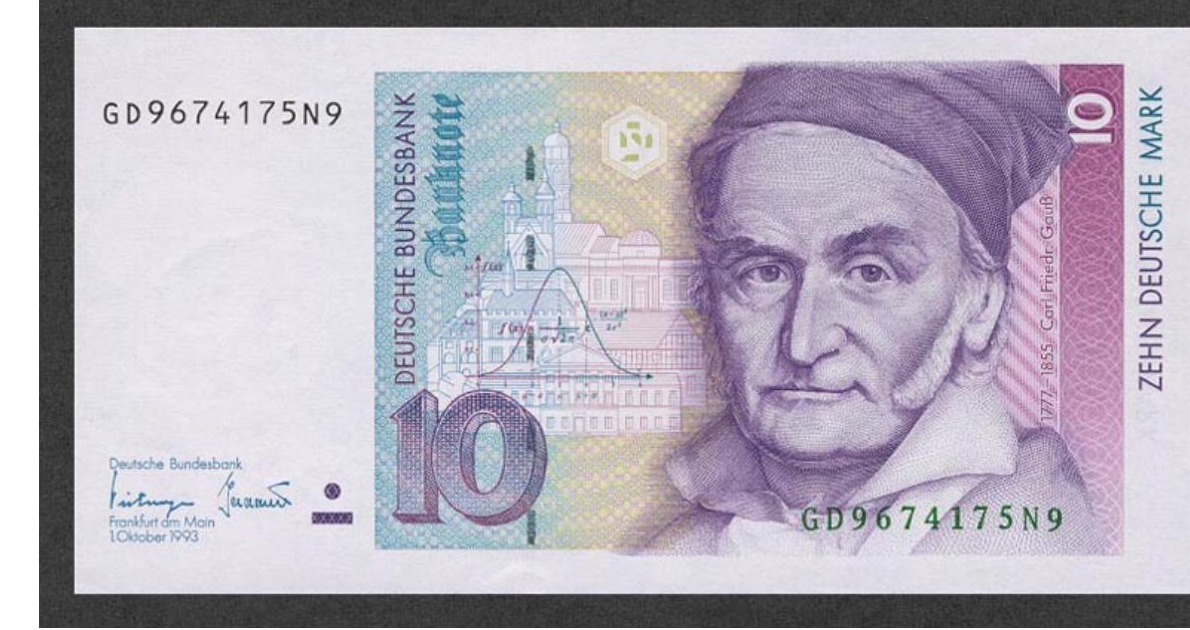
\includegraphics[width=0.9\textwidth]{images/gauss_10dm.jpg}
  \vfill
\end{frame}

\begin{frame}[t]{Propriétés de la densité $N(\mu, \sigma^2)$}
  \begin{columns}[T]
    \column{0.5\textwidth}
      \begin{itemize}\itemsep 2mm
        \item $f(x) > 0$ pour tout $x$ et l'aire totale vaut 1;
        \item cloche \alert{symétrique} autour de $\mu$ :
          $f(\mu - x) = f(\mu + x)$;
        \item maximum unique en $x = \mu$;
        \item deux points d'inflexion, en $\mu - \sigma$ et $\mu + \sigma$.
      \end{itemize}
    \column{0.48\textwidth}
      \begin{tikzpicture}
        \begin{axis}[base, width=\linewidth, height=0.55\textheight,
            axis lines=left, ytick=\empty, xtick={-1,0,1},
            xticklabels={$\mu-\sigma$, $\mu$, $\mu+\sigma$},
            ymin=0, ymax=0.45, domain=-3.5:3.5, samples=100]
          \addplot[thick, Accent] {exp(-x^2/2)/sqrt(2*pi)};
          \addplot[dashed, gray] coordinates {(0,0) (0,0.399)};
          \addplot[only marks, mark=*, mark size=1.5pt, Dominante!80!black]
            coordinates {(-1,0.242) (1,0.242)};
        \end{axis}
      \end{tikzpicture}
  \end{columns}

  \medskip
  \uncover<2->{
  Mais la fonction de répartition
  $F(x) = \int_{-\infty}^{x} \frac{1}{\sigma\sqrt{2\pi}} e^{-\frac{1}{2}\left(\frac{t-\mu}{\sigma}\right)^2} dt$
  \alert{n'a pas de forme explicite} : on utilise un logiciel (R) ou une table.
  }
\end{frame}

\begin{frame}[plain,t]
  \centerline{\LARGE\bfseries\alert{QUIZ !}}

  \medskip
  Le poids à la naissance $X$ (en g) des bébés nés à terme suit
  approximativement une loi normale de paramètres $\mu = 3400$\,g et
  $\sigma^2 = 500^2$\,g$^2$. Sans faire de calcul, répondez :
  \begin{enumerate}\itemsep 1cm
    \item Laquelle est la plus grande : $P(X < 2400)$ ou $P(X > 4400)$?
    \item Laquelle est la plus grande : $P(2400 < X < 2500)$ ou
      $P(3400 < X < 3500)$?
    \item Si l'écart type était plutôt de 400\,g (même moyenne),
      $P(X < 2400)$ augmenterait-elle ou diminuerait-elle?
  \end{enumerate}
\end{frame}

\begin{frame}[t]{Loi normale standard}
  \begin{Boite}{Loi normale standard (centrée réduite)}
    La loi $N(0, 1)$ est appelée \alert{loi normale standard}. Si
    $Z \sim N(0, 1)$, on note $\Phi(z) = P(Z \le z)$ sa fonction de
    répartition.
  \end{Boite}

  \begin{columns}[c]
    \column{0.5\textwidth}
      Par symétrie de la densité autour de 0 :
      \[ \Phi(-z) = 1 - \Phi(z). \]
      Les tables donnent donc $\Phi(z)$ seulement pour $z \ge 0$.
    \column{0.48\textwidth}
      \begin{tikzpicture}
        \begin{axis}[base, width=\linewidth, height=0.45\textheight,
            axis lines=left, ytick=\empty, xtick={-1.2,0,1.2},
            xticklabels={$-z$, 0, $z$}, ymin=0, ymax=0.45, samples=80]
          \addplot[fill=Dominante!40, draw=none, domain=-3.5:-1.2] {exp(-x^2/2)/sqrt(2*pi)} \closedcycle;
          \addplot[fill=Accent!40, draw=none, domain=1.2:3.5] {exp(-x^2/2)/sqrt(2*pi)} \closedcycle;
          \addplot[thick, black, domain=-3.5:3.5] {exp(-x^2/2)/sqrt(2*pi)};
        \end{axis}
      \end{tikzpicture}
  \end{columns}
\end{frame}

\begin{frame}[t]{Table de la loi normale standard :
    $\Phi(z) = \int_{-\infty}^{z} \frac{1}{\sqrt{2\pi}} e^{-x^2/2}\,dx$}
  \centering\tiny
  \renewcommand{\arraystretch}{0.95}
  \setlength{\tabcolsep}{4pt}
  \begin{tabular}{c|cccccccccc}
    \toprule
    $z$ & 0.00 & 0.01 & 0.02 & 0.03 & 0.04 & 0.05 & 0.06 & 0.07 & 0.08 & 0.09 \\
    \midrule
0.0 & 0.5000 & 0.5040 & 0.5080 & 0.5120 & 0.5160 & 0.5199 & 0.5239 & 0.5279 & 0.5319 & 0.5359 \\
0.1 & 0.5398 & 0.5438 & 0.5478 & 0.5517 & 0.5557 & 0.5596 & 0.5636 & 0.5675 & 0.5714 & 0.5753 \\
0.2 & 0.5793 & 0.5832 & 0.5871 & 0.5910 & 0.5948 & 0.5987 & 0.6026 & 0.6064 & 0.6103 & 0.6141 \\
0.3 & 0.6179 & 0.6217 & 0.6255 & 0.6293 & 0.6331 & 0.6368 & 0.6406 & 0.6443 & 0.6480 & 0.6517 \\
0.4 & 0.6554 & 0.6591 & 0.6628 & 0.6664 & 0.6700 & 0.6736 & 0.6772 & 0.6808 & 0.6844 & 0.6879 \\
\midrule
0.5 & 0.6915 & 0.6950 & 0.6985 & 0.7019 & 0.7054 & 0.7088 & 0.7123 & 0.7157 & 0.7190 & 0.7224 \\
0.6 & 0.7257 & 0.7291 & 0.7324 & 0.7357 & 0.7389 & 0.7422 & 0.7454 & 0.7486 & 0.7517 & 0.7549 \\
0.7 & 0.7580 & 0.7611 & 0.7642 & 0.7673 & 0.7704 & 0.7734 & 0.7764 & 0.7794 & 0.7823 & 0.7852 \\
0.8 & 0.7881 & 0.7910 & 0.7939 & 0.7967 & 0.7995 & 0.8023 & 0.8051 & 0.8078 & 0.8106 & 0.8133 \\
0.9 & 0.8159 & 0.8186 & 0.8212 & 0.8238 & 0.8264 & 0.8289 & 0.8315 & 0.8340 & 0.8365 & 0.8389 \\
\midrule
1.0 & 0.8413 & 0.8438 & 0.8461 & 0.8485 & 0.8508 & 0.8531 & 0.8554 & 0.8577 & 0.8599 & 0.8621 \\
1.1 & 0.8643 & 0.8665 & 0.8686 & 0.8708 & 0.8729 & 0.8749 & 0.8770 & 0.8790 & 0.8810 & 0.8830 \\
1.2 & 0.8849 & 0.8869 & 0.8888 & 0.8907 & 0.8925 & 0.8944 & 0.8962 & 0.8980 & 0.8997 & 0.9015 \\
1.3 & 0.9032 & 0.9049 & 0.9066 & 0.9082 & 0.9099 & 0.9115 & 0.9131 & 0.9147 & 0.9162 & 0.9177 \\
1.4 & 0.9192 & 0.9207 & 0.9222 & 0.9236 & 0.9251 & 0.9265 & 0.9279 & 0.9292 & 0.9306 & 0.9319 \\
\midrule
1.5 & 0.9332 & 0.9345 & 0.9357 & 0.9370 & 0.9382 & 0.9394 & 0.9406 & 0.9418 & 0.9429 & 0.9441 \\
1.6 & 0.9452 & 0.9463 & 0.9474 & 0.9484 & 0.9495 & 0.9505 & 0.9515 & 0.9525 & 0.9535 & 0.9545 \\
1.7 & 0.9554 & 0.9564 & 0.9573 & 0.9582 & 0.9591 & 0.9599 & 0.9608 & 0.9616 & 0.9625 & 0.9633 \\
    \bottomrule
  \end{tabular}
\end{frame}

\begin{frame}[t]{Table de la loi normale standard (suite)}
  \centering\tiny
  \renewcommand{\arraystretch}{0.95}
  \setlength{\tabcolsep}{4pt}
  \begin{tabular}{c|cccccccccc}
    \toprule
    $z$ & 0.00 & 0.01 & 0.02 & 0.03 & 0.04 & 0.05 & 0.06 & 0.07 & 0.08 & 0.09 \\
    \midrule
1.8 & 0.9641 & 0.9649 & 0.9656 & 0.9664 & 0.9671 & 0.9678 & 0.9686 & 0.9693 & 0.9699 & 0.9706 \\
1.9 & 0.9713 & 0.9719 & 0.9726 & 0.9732 & 0.9738 & 0.9744 & 0.9750 & 0.9756 & 0.9761 & 0.9767 \\
\midrule
2.0 & 0.9772 & 0.9778 & 0.9783 & 0.9788 & 0.9793 & 0.9798 & 0.9803 & 0.9808 & 0.9812 & 0.9817 \\
2.1 & 0.9821 & 0.9826 & 0.9830 & 0.9834 & 0.9838 & 0.9842 & 0.9846 & 0.9850 & 0.9854 & 0.9857 \\
2.2 & 0.9861 & 0.9864 & 0.9868 & 0.9871 & 0.9875 & 0.9878 & 0.9881 & 0.9884 & 0.9887 & 0.9890 \\
2.3 & 0.9893 & 0.9896 & 0.9898 & 0.9901 & 0.9904 & 0.9906 & 0.9909 & 0.9911 & 0.9913 & 0.9916 \\
2.4 & 0.9918 & 0.9920 & 0.9922 & 0.9925 & 0.9927 & 0.9929 & 0.9931 & 0.9932 & 0.9934 & 0.9936 \\
\midrule
2.5 & 0.9938 & 0.9940 & 0.9941 & 0.9943 & 0.9945 & 0.9946 & 0.9948 & 0.9949 & 0.9951 & 0.9952 \\
2.6 & 0.9953 & 0.9955 & 0.9956 & 0.9957 & 0.9959 & 0.9960 & 0.9961 & 0.9962 & 0.9963 & 0.9964 \\
2.7 & 0.9965 & 0.9966 & 0.9967 & 0.9968 & 0.9969 & 0.9970 & 0.9971 & 0.9972 & 0.9973 & 0.9974 \\
2.8 & 0.9974 & 0.9975 & 0.9976 & 0.9977 & 0.9977 & 0.9978 & 0.9979 & 0.9979 & 0.9980 & 0.9981 \\
2.9 & 0.9981 & 0.9982 & 0.9982 & 0.9983 & 0.9984 & 0.9984 & 0.9985 & 0.9985 & 0.9986 & 0.9986 \\
\midrule
3.0 & 0.9987 & 0.9987 & 0.9987 & 0.9988 & 0.9988 & 0.9989 & 0.9989 & 0.9989 & 0.9990 & 0.9990 \\
3.1 & 0.9990 & 0.9991 & 0.9991 & 0.9991 & 0.9992 & 0.9992 & 0.9992 & 0.9992 & 0.9993 & 0.9993 \\
3.2 & 0.9993 & 0.9993 & 0.9994 & 0.9994 & 0.9994 & 0.9994 & 0.9994 & 0.9995 & 0.9995 & 0.9995 \\
3.3 & 0.9995 & 0.9995 & 0.9995 & 0.9996 & 0.9996 & 0.9996 & 0.9996 & 0.9996 & 0.9996 & 0.9997 \\
3.4 & 0.9997 & 0.9997 & 0.9997 & 0.9997 & 0.9997 & 0.9997 & 0.9997 & 0.9997 & 0.9997 & 0.9998 \\
\midrule
3.5 & 0.9998 & 0.9998 & 0.9998 & 0.9998 & 0.9998 & 0.9998 & 0.9998 & 0.9998 & 0.9998 & 0.9998 \\
3.6 & 0.9998 & 0.9998 & 0.9999 & 0.9999 & 0.9999 & 0.9999 & 0.9999 & 0.9999 & 0.9999 & 0.9999 \\
    \bottomrule
  \end{tabular}

  \bigskip
  \begin{tabular}{c|cccccccccc}
    \toprule
    $\Phi(z)$ & 0.80 & 0.90 & 0.95 & 0.975 & 0.98 & 0.99 & 0.995 & 0.9975 & 0.999 & 0.9995 \\
    $z$ & 0.841 & 1.282 & 1.645 & 1.960 & 2.054 & 2.326 & 2.576 & 2.807 & 3.091 & 3.291 \\
    \bottomrule
  \end{tabular}
\end{frame}

\begin{frame}[plain,t]
  \centerline{\LARGE\bfseries\alert{QUIZ !}}

  \medskip
  Soit $Z \sim N(0, 1)$. À l'aide de la table, trouvez :
  \begin{columns}[T]
    \column{0.5\textwidth}
      \begin{enumerate}[a)]\itemsep 5mm
        \item $P(Z < 1.15)$
        \item $P(Z > 1.15)$
        \item $P(0.4 < Z < 2.12)$
        \item $P(Z < -1.4)$
      \end{enumerate}
    \column{0.5\textwidth}
      \begin{enumerate}[a)]\itemsep 5mm
        \setcounter{enumi}{4}
        \item $P(|Z| < 2)$
        \item la valeur $c$ telle que $P(Z < c) = 0.78$
        \item la valeur $c$ telle que $P(Z > c) = 0.025$
      \end{enumerate}
  \end{columns}
\end{frame}

\begin{frame}[t]{Standardisation}
  \begin{thm}
    \[
      X \sim N(\mu, \sigma^2) \quad \Longrightarrow \quad
      Z = \frac{X - \mu}{\sigma} \sim N(0, 1)
    \]
  \end{thm}
  $\Rightarrow$ Une seule table (celle de la $N(0, 1)$) suffit!

  \medskip
  \uncover<2->{
  \[
    P(a < X \le b) = P\left(\frac{a - \mu}{\sigma} < Z \le \frac{b - \mu}{\sigma}\right)
    = \Phi\left(\frac{b - \mu}{\sigma}\right) - \Phi\left(\frac{a - \mu}{\sigma}\right).
  \]
  }
  \uncover<3->{
  Un calcul de probabilité pour une loi normale se fait donc en deux étapes :
  \begin{enumerate}
    \item \alert{standardiser} la v.a.\ d'intérêt pour se ramener à la $N(0, 1)$;
    \item aller chercher les valeurs de $\Phi(\cdot)$ dans la table (ou dans R).
  \end{enumerate}
  }
\end{frame}

\begin{frame}[t]{Standardisation : centrer, puis réduire}
  \begin{columns}[T]
    \column{0.56\textwidth}
      \begin{enumerate}\itemsep 2mm
        \item \alert{Centrer} : $X - \mu \sim N(0, \sigma^2)$.\\
          {\small On déplace la cloche pour qu'elle soit centrée en 0.}
        \item \alert{Réduire} : $\dfrac{X - \mu}{\sigma} \sim N(0, 1)$.\\
          {\small On change d'unité : la nouvelle unité est l'écart type.}
      \end{enumerate}
    \column{0.42\textwidth}
      \begin{tikzpicture}
        \begin{axis}[base, width=\linewidth, height=0.38\textheight,
            axis lines=left, ytick=\empty, ymin=0, ymax=0.45, xmin=-7, xmax=11,
            xtick={0,4}, samples=100,
            legend style={font=\tiny, draw=none, fill=none, at={(0.5,1.03)}, anchor=south},
            legend columns=3, legend cell align=left]
          \addplot[thick, black, dotted, domain=-2:10] {exp(-(x-4)^2/8)/(2*sqrt(2*pi))};
          \addplot[thick, Dominante!80!black, dashed, domain=-6:6] {exp(-x^2/8)/(2*sqrt(2*pi))};
          \addplot[thick, Accent, domain=-4:4] {exp(-x^2/2)/sqrt(2*pi)};
          \legend{{$N(4, 2^2)$}, {$N(0, 2^2)$}, {$N(0, 1)$}}
        \end{axis}
      \end{tikzpicture}
  \end{columns}

  \smallskip
  \textbf{Justification.} $Z = \frac{1}{\sigma} X - \frac{\mu}{\sigma}$ est de
  la forme $aX + b$. Par les propriétés de la 1\textsuperscript{re} partie,
  $E(Z) = \frac{E(X) - \mu}{\sigma} = 0$ et
  $\operatorname{Var}(Z) = \frac{\operatorname{Var}(X)}{\sigma^2} = 1$; de
  plus, une transformation linéaire d'une v.a.\ normale est encore normale.

  \smallskip
  \textbf{Interprétation.} $z = (x - \mu)/\sigma$ est le \alert{nombre
  d'écarts types} qui séparent $x$ de la moyenne. Ex. : un bébé de 2\,650\,g a
  $z = (2650 - 3400)/500 = -1.5$.
\end{frame}

\begin{frame}[t]{Règle empirique : 68 -- 95 -- 99.7}
  \begin{columns}[c]
    \column{0.5\textwidth}
      \begin{Boite}{Règle empirique}
        Si $X \sim N(\mu, \sigma^2)$, environ
        \begin{itemize}
          \item \alert{68\,\%} des valeurs sont dans $\mu \pm \sigma$;
          \item \alert{95\,\%} sont dans $\mu \pm 2\sigma$;
          \item \alert{99.7\,\%} sont dans $\mu \pm 3\sigma$.
        \end{itemize}
      \end{Boite}
    \column{0.48\textwidth}
      \begin{tikzpicture}
        \begin{axis}[base, width=\linewidth, height=0.44\textheight,
            axis lines=left, ytick=\empty, ymin=0, ymax=0.45, xmin=-3.6, xmax=3.6,
            xtick={-3,-2,-1,0,1,2,3}, samples=60,
            xticklabels={$-3\sigma$, $-2\sigma$, $-\sigma$, $\mu$, $\sigma$, $2\sigma$, $3\sigma$},
            xticklabel style={font=\tiny}]
          \addplot[fill=Dominante!15, draw=none, domain=-3:3] {exp(-x^2/2)/sqrt(2*pi)} \closedcycle;
          \addplot[fill=Dominante!35, draw=none, domain=-2:2] {exp(-x^2/2)/sqrt(2*pi)} \closedcycle;
          \addplot[fill=Dominante!65, draw=none, domain=-1:1] {exp(-x^2/2)/sqrt(2*pi)} \closedcycle;
          \addplot[thick, black, domain=-3.6:3.6] {exp(-x^2/2)/sqrt(2*pi)};
          \node[font=\tiny] at (axis cs:0,0.15) {68\,\%};
          \node[font=\tiny] at (axis cs:-1.5,0.03) {95\,\%};
          \node[font=\tiny] at (axis cs:2.6,0.05) {99.7\,\%};
        \end{axis}
      \end{tikzpicture}
  \end{columns}

  {\scriptsize\color{gray} Valeurs exactes : $\Phi(1) - \Phi(-1) = 0.6827$,
  $\Phi(2) - \Phi(-2) = 0.9545$, $\Phi(3) - \Phi(-3) = 0.9973$. Pour
  exactement 95\,\%, il faut $\pm 1.96\,\sigma$.}

  \smallskip
  \textbf{Poids à la naissance} ($\mu = 3400$\,g, $\sigma = 500$\,g) : environ
  68\,\% des bébés pèsent entre 2\,900 et 3\,900\,g, 95\,\% entre 2\,400 et
  4\,400\,g, et presque tous (99.7\,\%) entre 1\,900 et 4\,900\,g. Une valeur à
  plus de 3 écarts types de la moyenne est donc \alert{très inhabituelle}.
\end{frame}

\begin{frame}[t]{Exemple 4}
  La taille d'une fille de 12 mois ($X$) suit une distribution normale de
  moyenne 74\,cm et de variance 9\,cm$^2$ : $X \sim N(74, 9)$.

  \begin{enumerate}[a)]\itemsep 1.2cm
    \item À 12 mois, une fillette mesure 71\,cm. Quelle proportion des
      fillettes sont plus petites qu'elle?
    \item Quelle est la probabilité qu'une fillette choisie au hasard mesure
      entre 70 et 75\,cm?
    \item On considère que les 1\,\% des fillettes les plus petites devraient
      faire l'objet d'un suivi spécial. À partir de quelle taille les
      fillettes doivent-elles faire l'objet d'un suivi?
  \end{enumerate}
\end{frame}

\begin{frame}[t]{Exemple 4 : commencer par un croquis}
  \centering
  \begin{tikzpicture}
    \begin{axis}[base, width=0.8\textwidth, height=0.6\textheight,
        axis lines=left, ytick=\empty, xtick={65,68,71,74,77,80,83},
        xlabel={Taille (cm)}, ymin=0, ymax=0.14, samples=100]
      \only<1>{\addplot[fill=Dominante!40, draw=none, domain=64:71] {exp(-(x-74)^2/18)/(3*sqrt(2*pi))} \closedcycle;}
      \only<2| handout:0>{\addplot[fill=Dominante!40, draw=none, domain=70:75] {exp(-(x-74)^2/18)/(3*sqrt(2*pi))} \closedcycle;}
      \only<3| handout:0>{\addplot[fill=Accent!50, draw=none, domain=64:67.02] {exp(-(x-74)^2/18)/(3*sqrt(2*pi))} \closedcycle;}
      \addplot[thick, black, domain=64:84] {exp(-(x-74)^2/18)/(3*sqrt(2*pi))};
    \end{axis}
  \end{tikzpicture}

  \raggedright
  \only<1>{a) $P(X < 71)$ : aire à gauche de 71, soit à $\sigma = 3$ sous la moyenne.}
  \only<2| handout:0>{b) $P(70 < X < 75)$ : aire entre 70 et 75.}
  \only<3| handout:0>{c) On cherche $x^*$ tel que l'aire à gauche de $x^*$ vaut 0.01.}
\end{frame}

\begin{frame}[fragile,t]{Exemple 4 : calculs dans R}
  \begin{itemize}\itemsep 2mm
    \item a) $P(X < 71)$
\begin{console}
> pnorm(71, mean = 74, sd = 3)
[1] 0.1586553
\end{console}
    \item b) $P(70 \le X \le 75)$
\begin{console}
> pnorm(75, mean = 74, sd = 3) - pnorm(70, mean = 74, sd = 3)
[1] 0.5393474
\end{console}
    \item c) Pour quel $x^*$ a-t-on $P(X \le x^*) = 0.01$?
\begin{console}
> qnorm(0.01, mean = 74, sd = 3)
[1] 67.02096
\end{console}
  \end{itemize}
  {\small\color{gray} Attention : dans R, on donne l'écart type \texttt{sd}, pas la variance!}
\end{frame}

\begin{frame}[plain,t]
  \centerline{\LARGE\bfseries\alert{QUIZ !}}

  \medskip
  Chez les adultes en santé, la glycémie à jeun $X$ (en mmol/L) suit
  approximativement une loi $N(5.0,\; 0.5^2)$.
  \begin{itemize}\itemsep 1.1cm
    \item Un patient a une glycémie de 6.1\,mmol/L. À combien d'écarts types
      de la moyenne se situe-t-il?
    \item Quelle proportion des adultes en santé ont une glycémie
      supérieure à la sienne?
    \item Sous quelle valeur se trouve la glycémie de 95\,\% des adultes
      en santé?
  \end{itemize}
\end{frame}

\begin{frame}[t]{Combinaisons linéaires de v.a.\ normales}
  \begin{prp}
    \begin{enumerate}\itemsep 2mm
      \item Si $X \sim N(\mu, \sigma^2)$ et $Y = aX + b$, alors
        $Y \sim N(a\mu + b,\; a^2\sigma^2)$.
      \item Si $X_1, \ldots, X_n$ sont \alert{indépendantes} avec
        $X_i \sim N(\mu_i, \sigma_i^2)$, alors
        \[
          a_1 X_1 + \cdots + a_n X_n \sim
          N\big(a_1\mu_1 + \cdots + a_n\mu_n,\;\; a_1^2\sigma_1^2 + \cdots + a_n^2\sigma_n^2\big).
        \]
    \end{enumerate}
  \end{prp}

  \uncover<2->{
  Cas particuliers importants ($X$ et $Y$ normales \alert{indépendantes}) :
  \[
    X + Y \sim N(\mu_X + \mu_Y,\; \sigma_X^2 + \sigma_Y^2), \qquad
    X - Y \sim N(\mu_X - \mu_Y,\; \sigma_X^2 + \sigma_Y^2).
  \]
  {\small \alert{Attention !} La variance d'une \emph{différence} est une
  \emph{somme} : $\operatorname{Var}(X - Y) = 1^2\sigma_X^2 + (-1)^2\sigma_Y^2$.
  Soustraire deux quantités aléatoires ajoute de l'incertitude, ça ne
  l'enlève pas. \color{gray}(Utile au chapitre 4 pour comparer deux
  moyennes.)}
  }
\end{frame}

\begin{frame}[t]{Exemple 5}
  La masse d'une orange est une variable aléatoire \textbf{de distribution
  normale} d'espérance 204\,g et de variance 256\,g$^2$. On crée des sacs de 7
  oranges. La masse de l'emballage est une variable normale de moyenne 50\,g
  et de variance 10\,g$^2$. Toutes ces masses sont indépendantes.

  \medskip
  Quelle est la probabilité que la masse d'un sac choisi au hasard soit
  inférieure à 1400\,g?

  \vspace{2.5cm}
  {\small\color{gray} Rappel : on a calculé l'espérance et la variance d'un sac
  de 7 oranges à la fin de la 1\textsuperscript{re} partie. Ce qui est
  nouveau : on connaît maintenant la \emph{loi} de la masse du sac.}
\end{frame}

\begin{frame}[t]{Exemple 6}
  Dans une animalerie, la masse (en g) des souris adultes d'une lignée suit une
  loi $N(30,\; 9)$ chez les mâles et une loi $N(26,\; 7)$ chez les femelles.
  On choisit au hasard un mâle et une femelle, dont les masses $M$ et $F$ sont
  indépendantes.

  \medskip
  \alert{Quelle est la probabilité que la femelle soit plus lourde que le mâle?}

  \vspace{2.5cm}
  {\small\color{gray} Piste : $P(F > M) = P(F - M > 0)$. Quelle est la loi de $D = F - M$?}
\end{frame}

\begin{frame}[t]{Et si les v.a.\ ne sont pas indépendantes?}
  Les formules de variance précédentes supposent l'\alert{indépendance}. Sinon,
  il faut tenir compte de la \alert{covariance} :
  \[
    \operatorname{Var}(X \pm Y) = \operatorname{Var}(X) + \operatorname{Var}(Y)
    \pm 2\operatorname{Cov}(X, Y),
    \qquad \operatorname{Cov}(X, Y) = E\big[(X - \mu_X)(Y - \mu_Y)\big].
  \]
  \vspace{-2mm}
  \begin{itemize}\itemsep 1.5mm\small
    \item $\operatorname{Cov}(X, Y) > 0$ : $X$ et $Y$ ont tendance à être
      grandes (ou petites) \emph{en même temps} (ex. : longueur et masse d'un
      poisson).
    \item $\operatorname{Cov}(X, Y) < 0$ : quand l'une est grande, l'autre a
      tendance à être petite.
    \item La \alert{corrélation}
      $\rho = \operatorname{Cov}(X, Y) / (\sigma_X \sigma_Y)$ est sans unité et
      toujours entre $-1$ et $1$.
    \item Si $X$ et $Y$ sont indépendantes, alors $\operatorname{Cov}(X, Y) = 0$
      (mais la réciproque est fausse).
  \end{itemize}

  \medskip
  {\small\color{gray} Dans ce cours, on supposera presque toujours
  l'indépendance. On retrouvera ces idées avec les données appariées
  (chapitre 4) et la corrélation échantillonnale (chapitre 6).}
\end{frame}

%===============================================================================
\section[TLC]{Le théorème limite central}
%===============================================================================

\begin{frame}[t]{Exemple exploratoire}
  $\mathcal{E}$ : lancer deux dés ($n = 2$) et faire la somme.
  On répète l'expérience 1000 fois.

  \begin{columns}[T]
    \column{0.36\textwidth}
      \footnotesize Extrait des résultats

      \scriptsize
      \renewcommand{\arraystretch}{0.9}
      \begin{tabular}{ccc}
        \toprule
        $X_1$ & $X_2$ & $S = X_1 + X_2$ \\
        \midrule
        6 & 4 & 10 \\ 3 & 2 & 5 \\ 4 & 1 & 5 \\ 3 & 1 & 4 \\
        5 & 6 & 11 \\ 6 & 6 & 12 \\ 3 & 5 & 8 \\ 6 & 1 & 7 \\
        3 & 5 & 8 \\ 1 & 3 & 4 \\ 1 & 5 & 6 \\ 1 & 1 & 2 \\
        \bottomrule
      \end{tabular}
    \column{0.62\textwidth}
      \pgfplotsset{des/.style={ybar, bar width=0.6, width=\linewidth, height=0.29\textheight,
          ymin=0, ymax=200, ytick={0,100,200}, tick label style={font=\tiny},
          label style={font=\scriptsize}, ylabel={Fréq.}, ylabel style={yshift=-3mm}}}
      \begin{tikzpicture}
        \begin{axis}[des, xlabel={$X_1$}, xtick={1,...,6}, xlabel style={yshift=2mm}]
          \addplot[fill=Dominante, draw=none] coordinates {(1,171) (2,149) (3,187) (4,145) (5,181) (6,167)};
        \end{axis}
      \end{tikzpicture}

      \vspace{-2mm}
      \begin{tikzpicture}
        \begin{axis}[des, xlabel={$X_2$}, xtick={1,...,6}, xlabel style={yshift=2mm}]
          \addplot[fill=Dominante, draw=none] coordinates {(1,168) (2,171) (3,170) (4,139) (5,181) (6,171)};
        \end{axis}
      \end{tikzpicture}

      \vspace{-2mm}
      \begin{tikzpicture}
        \begin{axis}[des, xlabel={$S$}, xtick={2,...,12}, xlabel style={yshift=2mm}]
          \addplot[fill=Accent, draw=none] coordinates {(2,29) (3,55) (4,86) (5,101) (6,137) (7,189) (8,112) (9,121) (10,76) (11,66) (12,28)};
        \end{axis}
      \end{tikzpicture}
  \end{columns}
\end{frame}

\begin{frame}[plain,t]
  \centerline{\LARGE\bfseries\alert{QUIZ !}}

  \medskip
  Une urne contient 3 boules numérotées 1, 2, 3. On pige une boule, on la
  remet, puis on en pige une autre. Vrai ou faux?

  \medskip
  \begin{columns}[T]
    \column{0.48\textwidth}
      1) La valeur de la première boule a la distribution suivante :

      \begin{tikzpicture}
        \begin{axis}[petit, width=\linewidth, height=0.42\textheight,
            xtick={1,2,3}, xmin=0.5, xmax=3.5, ymax=0.45, ylabel={$p(x)$}]
          \addplot[batons] coordinates {(1,1/3) (2,1/3) (3,1/3)};
        \end{axis}
      \end{tikzpicture}
    \column{0.48\textwidth}
      2) La somme des deux numéros a la distribution suivante :

      \begin{tikzpicture}
        \begin{axis}[petit, width=\linewidth, height=0.42\textheight,
            xtick={2,...,6}, xmin=1.5, xmax=6.5, ymax=0.45, ylabel={$p(s)$}]
          \addplot[batons] coordinates {(2,1/5) (3,1/5) (4,1/5) (5,1/5) (6,1/5)};
        \end{axis}
      \end{tikzpicture}
  \end{columns}
\end{frame}

\begin{frame}[t]{Sommes de variables exponentielles}
  Même en partant d'une loi très asymétrique, la somme de plusieurs v.a.\
  indépendantes prend une forme de cloche.

  \centering
  \pgfplotsset{gam/.style={petit, height=0.36\textheight, xlabel={$x$}, ylabel={Densité}, samples=100, no markers}}
  \begin{tikzpicture}
    \begin{axis}[gam, title={1 exponentielle}, domain=0:5]
      \addplot[thick, Accent] {2*exp(-2*x)};
    \end{axis}
  \end{tikzpicture}\hfill
  \begin{tikzpicture}
    \begin{axis}[gam, title={Somme de 3}, domain=0:10]
      \addplot[thick, Accent] {2^3*x^2*exp(-2*x)/2};
    \end{axis}
  \end{tikzpicture}

  \begin{tikzpicture}
    \begin{axis}[gam, title={Somme de 12}, domain=0:12]
      \addplot[thick, Accent] {exp(12*ln(2) + 11*ln(max(x,1e-6)) - 2*x - 17.502308)};
    \end{axis}
  \end{tikzpicture}\hfill
  \begin{tikzpicture}
    \begin{axis}[gam, title={Somme de 30}, domain=0:25]
      \addplot[thick, Accent] {exp(30*ln(2) + 29*ln(max(x,1e-6)) - 2*x - 71.257039)};
    \end{axis}
  \end{tikzpicture}
\end{frame}

\begin{frame}[t]{Un résultat très (très) utile}
  \begin{thm}
    Soit $X_1, X_2, \ldots, X_n$ des variables aléatoires \alert{indépendantes
    et identiquement distribuées} de moyenne $\mu$ et de variance $\sigma^2$,
    de loi quelconque. Alors, si $n$ est assez grand,
    \begin{align*}
      S_n &= X_1 + X_2 + \cdots + X_n \;\approx\; N(n\mu,\; n\sigma^2)
      \quad \text{et} \\
      \overline{X} &= \frac{X_1 + X_2 + \cdots + X_n}{n} \;\approx\;
      N\!\left(\mu,\; \frac{\sigma^2}{n}\right).
    \end{align*}
  \end{thm}
  C'est le \alert{théorème limite central} (TLC).

  \medskip
  {\small\color{gray} L'espérance et la variance de $S_n$ et de
  $\overline{X}$ découlent des propriétés vues en 1\textsuperscript{re}
  partie; le TLC ajoute que la loi est \emph{à peu près normale}. En pratique,
  on considère souvent que $n \ge 30$ suffit.}
\end{frame}

\begin{frame}[t]{Le TLC en action : simulation}
  \small Temps d'attente $X$ (en min) entre deux visites de pollinisateurs
  sur une fleur : loi exponentielle, très asymétrique, avec $\mu = 2$ et
  $\sigma = 2$. On simule $10\,000$ échantillons de taille $n$ et on trace
  l'histogramme des $10\,000$ moyennes $\overline{X}$.
  \normalsize

  \smallskip
  \begin{columns}[T]
    \column{0.64\textwidth}
  \pgfplotsset{tlc/.style={base, width=0.56\linewidth, height=0.33\textheight,
      xmin=0, xmax=6, ymin=0, ymax=1.2, xtick={0,1,...,6}, ytick={0,0.5,1},
      tick label style={font=\tiny}, title style={font=\scriptsize\bfseries, yshift=-5pt},
      axis lines=left}}
  \centering
  \begin{tikzpicture}
    \begin{axis}[tlc, title={$n = 1$ \ (écart type 2)}]
      \addplot[ybar interval, fill=Dominante!45, draw=white, very thin] coordinates {(0,0.479) (0.2,0.426) (0.4,0.388) (0.6,0.342) (0.8,0.317) (1,0.272) (1.2,0.264) (1.4,0.249) (1.6,0.210) (1.8,0.194) (2,0.172) (2.2,0.164) (2.4,0.141) (2.6,0.138) (2.8,0.117) (3,0.102) (3.2,0.114) (3.4,0.088) (3.6,0.073) (3.8,0.065) (4,0.060) (4.2,0.058) (4.4,0.053) (4.6,0.051) (4.8,0.042) (5,0.040) (5.2,0.035) (5.4,0.032) (5.6,0.026) (5.8,0.030) (6,0)};
      \addplot[thick, Accent, domain=0:6] {0.5*exp(-x/2)};
    \end{axis}
  \end{tikzpicture}\hfill
  \begin{tikzpicture}
    \begin{axis}[tlc, title={$n = 5$ \ (écart type 0.89)}]
      \addplot[ybar interval, fill=Dominante!45, draw=white, very thin] coordinates {(0,0.001) (0.2,0.021) (0.4,0.076) (0.6,0.175) (0.8,0.284) (1,0.358) (1.2,0.453) (1.4,0.504) (1.6,0.462) (1.8,0.456) (2,0.427) (2.2,0.356) (2.4,0.315) (2.6,0.246) (2.8,0.201) (3,0.171) (3.2,0.116) (3.4,0.116) (3.6,0.075) (3.8,0.051) (4,0.045) (4.2,0.026) (4.4,0.021) (4.6,0.018) (4.8,0.007) (5,0.006) (5.2,0.004) (5.4,0.004) (5.6,0.001) (5.8,0.002) (6,0)};
      \addplot[thick, Accent, domain=0:6] {exp(-(x-2)^2/(2*0.8))/sqrt(2*pi*0.8)};
    \end{axis}
  \end{tikzpicture}

  \vspace{-1mm}
  \begin{tikzpicture}
    \begin{axis}[tlc, title={$n = 10$ \ (écart type 0.63)}]
      \addplot[ybar interval, fill=Dominante!45, draw=white, very thin] coordinates {(0,0.000) (0.2,0.000) (0.4,0.003) (0.6,0.033) (0.8,0.101) (1,0.258) (1.2,0.404) (1.4,0.598) (1.6,0.658) (1.8,0.652) (2,0.606) (2.2,0.477) (2.4,0.384) (2.6,0.268) (2.8,0.194) (3,0.127) (3.2,0.093) (3.4,0.057) (3.6,0.035) (3.8,0.024) (4,0.010) (4.2,0.007) (4.4,0.004) (4.6,0.003) (4.8,0.003) (5,0.001) (5.2,0.001) (5.4,0.001) (5.6,0.001) (5.8,0.000) (6,0)};
      \addplot[thick, Accent, domain=0:6] {exp(-(x-2)^2/(2*0.4))/sqrt(2*pi*0.4)};
    \end{axis}
  \end{tikzpicture}\hfill
  \begin{tikzpicture}
    \begin{axis}[tlc, title={$n = 30$ \ (écart type 0.37)}]
      \addplot[ybar interval, fill=Dominante!45, draw=white, very thin] coordinates {(0,0.000) (0.2,0.000) (0.4,0.000) (0.6,0.001) (0.8,0.002) (1,0.024) (1.2,0.148) (1.4,0.447) (1.6,0.855) (1.8,1.131) (2,0.981) (2.2,0.714) (2.4,0.401) (2.6,0.194) (2.8,0.070) (3,0.025) (3.2,0.007) (3.4,0.001) (3.6,0.001) (3.8,0.001) (4,0.000) (4.2,0.000) (4.4,0.000) (4.6,0.000) (4.8,0.000) (5,0.000) (5.2,0.000) (5.4,0.000) (5.6,0.000) (5.8,0.000) (6,0)};
      \addplot[thick, Accent, domain=0:6] {exp(-(x-2)^2/(2*0.133333))/sqrt(2*pi*0.133333)};
    \end{axis}
  \end{tikzpicture}
    \column{0.34\textwidth}
      \small
      Quand $n$ augmente :
      \begin{itemize}\itemsep 2mm
        \item le \alert{centre} reste à $\mu = 2$;
        \item l'\alert{étalement} diminue comme $\sigma/\sqrt{n}$;
        \item la \alert{forme} devient celle d'une cloche.
      \end{itemize}

      \smallskip
      {\scriptsize\color{gray} Courbe : densité de départ ($n = 1$),
      puis $N(\mu, \sigma^2/n)$ prédite par le TLC.}
  \end{columns}
\end{frame}

\begin{frame}[t]{Conditions d'application du TLC}
  \begin{itemize}\itemsep 1mm
    \item Les observations $X_1, \ldots, X_n$ sont \alert{indépendantes}
      (échantillon aléatoire) et de \alert{même loi}.
    \item $n$ est \alert{assez grand}. Règle du pouce : $n \ge 30$. Mais cela
      dépend de la loi de départ :
      \begin{itemize}\small
        \item à peu près symétrique : $n$ plus petit suffit (somme de 2 dés!);
        \item très asymétrique : il faut un $n$ plus grand.
      \end{itemize}
    \item Si les $X_i$ sont déjà \alert{normales}, $\overline{X}$ est
      \emph{exactement} normale pour tout $n$ (combinaison linéaire de normales
      indépendantes) : pas besoin du TLC.
  \end{itemize}

  \vspace{-2mm}
  \begin{Boite}{Attention : ce que le TLC ne dit pas}
    \small Le TLC porte sur la loi de la \alert{moyenne} (ou de la somme), pas sur
    celle des observations : peser 1\,000 bébés au lieu de 30 ne rend pas
    les poids individuels « plus normaux ».
  \end{Boite}
\end{frame}

\begin{frame}[plain,t]
  \centerline{\LARGE\bfseries\alert{QUIZ !}}

  \medskip
  Dans chaque cas, peut-on considérer que $\overline{X}$ suit
  (approximativement) une loi normale? Pourquoi?
  \begin{enumerate}[a)]\itemsep 5mm
    \item $\overline{X}$ = nombre moyen de colonies bactériennes sur 50 boîtes
      de Petri indépendantes (nombre par boîte $\sim$ Poisson(12)).
    \item $\overline{X}$ = glycémie moyenne de 4 patients choisis au hasard,
      la glycémie étant de loi normale.
    \item $\overline{X}$ = temps de survie moyen de 6 souris, le temps de
      survie ayant une loi très asymétrique.
    \item Vrai ou faux : avec $n = 500$ bébés, l'histogramme des 500 poids à
      la naissance ressemblera à une cloche grâce au TLC.
  \end{enumerate}
\end{frame}

\begin{frame}[t]{Exemple 7}
  On sait que la concentration d'atrazine (un herbicide) dans les étangs d'une
  région a une moyenne de 4\,mg/l et un écart type de 1,5\,mg/l. On prend un
  échantillon d'eau d'un litre dans 40 de ces étangs.

  \medskip
  Quelle est la probabilité que la concentration moyenne d'atrazine dans ces
  échantillons dépasse 4,2\,mg/l?

  \vspace{2.5cm}
  \uncover<2->{
  {\small\color{gray} La loi de la concentration dans un étang n'est pas
  donnée : c'est le TLC qui nous permet de conclure.}
  }
\end{frame}

\begin{frame}[t]{Application : approximation normale de la binomiale}
  Une v.a.\ binomiale est une somme de v.a.\ Bernoulli($p$) indépendantes :
  $X = Y_1 + \cdots + Y_n$. Par le TLC, si $n$ est grand,
  \[ \text{Binomiale}(n, p) \approx N\big(np,\; np(1-p)\big). \]
  \vspace{-4mm}
  {\small Règle pratique : l'approximation est bonne si $np \ge 5$ et
  $n(1-p) \ge 5$.}

  \bigskip


  \centering
  \begin{tikzpicture}
    \begin{axis}[petit, height=0.38\textheight, title={Binomiale(6, 0.2)}, ylabel={$p(x)$}]
      \addplot[batons] coordinates {(0,0.26214) (1,0.39322) (2,0.24576) (3,0.08192) (4,0.01536) (5,0.00154) (6,0.00006)};
    \end{axis}
  \end{tikzpicture}\hfill
  \begin{tikzpicture}
    \begin{axis}[petit, height=0.38\textheight, title={Binomiale(30, 0.2)}, ylabel={$p(x)$}, samples=100]
      \addplot[batons] coordinates {(0,0.00124) (1,0.00928) (2,0.03366) (3,0.07853) (4,0.13252) (5,0.17228) (6,0.17946) (7,0.15382) (8,0.11056) (9,0.06756) (10,0.03547) (11,0.01612) (12,0.00638) (13,0.00221) (14,0.00067) (15,0.00018) (16,0.00004) (17,0.00001) (18,0.00000) (19,0.00000) (20,0.00000) (21,0.00000) (22,0.00000) (23,0.00000) (24,0.00000) (25,0.00000) (26,0.00000) (27,0.00000) (28,0.00000) (29,0.00000) (30,0.00000)};
      \addplot[thin, black, domain=0:30] {exp(-(x-6)^2/(2*4.8))/sqrt(2*pi*4.8)};
    \end{axis}
  \end{tikzpicture}
\end{frame}

\begin{frame}[t]{Correction pour la continuité}
  La binomiale est \alert{discrète}, la normale est \alert{continue} : on
  améliore l'approximation en élargissant de $1/2$ de chaque côté.

  \begin{prp}
    Si $X \sim \text{Binomiale}(n, p)$ et $n$ est grand, pour des entiers
    $j \le \ell$,
    \[
      P(j \le X \le \ell) \approx
      \Phi\!\left(\frac{(\ell + \frac{1}{2}) - np}{\sqrt{np(1-p)}}\right) -
      \Phi\!\left(\frac{(j - \frac{1}{2}) - np}{\sqrt{np(1-p)}}\right).
    \]
  \end{prp}

  \centering
  \begin{tikzpicture}
    \begin{axis}[base, width=0.55\textwidth, height=0.3\textheight,
        ymin=0, xmin=1.5, xmax=10.5, xtick={2,...,10},
        ytick=\empty, axis lines=left, samples=80]
      \addplot[ybar, bar width=1, bar shift=0pt, fill=gray!20, draw=gray] coordinates {(0,0.00080) (1,0.00684) (2,0.02785) (3,0.07160) (4,0.13042) (5,0.17886) (6,0.19164) (7,0.16426) (8,0.11440) (9,0.06537) (10,0.03082)};
      \addplot[ybar, bar width=1, bar shift=0pt, fill=Dominante!50, draw=gray] coordinates {(5,0.1789) (6,0.1916) (7,0.1643)};
      \addplot[thick, Accent, domain=1.5:10.5, smooth] {exp(-(x-6)^2/(2*4.2))/sqrt(2*pi*4.2)};
      \draw[dashed] (axis cs:4.5,0) -- (axis cs:4.5,0.2);
      \draw[dashed] (axis cs:7.5,0) -- (axis cs:7.5,0.2);
    \end{axis}
  \end{tikzpicture}

  {\scriptsize $P(5 \le X \le 7)$ : on intègre la densité normale de 4.5 à 7.5.}
\end{frame}

\begin{frame}[t]{Exemple 8}
  Environ 40\,\% des étudiants de la FSG ont déjà suivi un cours de
  statistique avant d'entrer à l'université. Sur la cohorte de 400 étudiants
  admis l'an dernier, quelle est la probabilité qu'entre 150 et 160 étudiants
  (inclusivement) aient déjà fait un cours de statistique?
\end{frame}

\begin{frame}[fragile,t]{Exemple 8 : vérification dans R}
  Valeur exacte (binomiale) :
\begin{console}
> sum(dbinom(150:160, size = 400, prob = 0.4))
[1] 0.3798861
\end{console}

  Approximation normale ($np = 160$, $np(1-p) = 96$), avec correction pour
  la continuité :
\begin{console}
> pnorm(160.5, 160, sqrt(96)) - pnorm(149.5, 160, sqrt(96))
[1] 0.3784114
\end{console}

  \ldots\ et sans correction pour la continuité :
\begin{console}
> pnorm(160, 160, sqrt(96)) - pnorm(150, 160, sqrt(96))
[1] 0.3462829
\end{console}
  {\small\color{gray} Avec la correction, l'erreur est d'environ 0.0015;
  sans elle, d'environ 0.034. La correction vaut la peine!}
\end{frame}

%-------------------------------------------------------------------------------
\begin{frame}[t]{Réponses aux exemples}
  \scriptsize
  \begin{columns}[T]
    \column{0.5\textwidth}
      \textbf{Loi de Bernoulli :} $E(Y) = p$, $\operatorname{Var}(Y) = p(1-p)$.

      \smallskip
      \textbf{Coefficient binomial :} $\binom{5}{2} = 10$;
      $\binom{49}{6} = 13\,983\,816$.

      \smallskip
      \textbf{Exemple 1 :} $X \sim \text{Bin}(5, 0.85)$;
      $P(X = 4) = 5 \times 0.85^4 \times 0.15 = 0.3915$.

      \smallskip
      \textbf{Quiz (fibrose kystique) :} $X \sim \text{Bin}(4, 0.25)$;
      $E(X) = 1$; $P(X = 0) = 0.75^4 = 0.3164$.

      \smallskip
      \textbf{Exemple 2 :} a) $P(X > 5) = 0.9556$; b) $np = 6.65$;
      c) $\sqrt{7(0.95)(0.05)} = 0.577$.

      \smallskip
      \textbf{Exemple 3 :} a) $P(X \le 2) = 0.1247$ ($\lambda = 5$);
      b) $P(X = 45) = 0.0458$ ($\lambda = 50$).

      \smallskip
      \textbf{Quiz (mutations) :} $\text{Bin}(300\,000,\ 10^{-5}) \approx
      \text{Poisson}(3)$; $P(X \ge 1) = 1 - e^{-3} = 0.9502$.

      \smallskip
      \textbf{Quiz (binomiale ou Poisson?) :} a) binomiale$(20, p)$;
      b) Poisson; c) binomiale$(1500,\ 10^{-4}) \approx$ Poisson$(0.15)$;
      d) ni l'une ni l'autre (v.a.\ continue, plutôt normale); e) ni l'une ni
      l'autre (contagion : les porcelets ne sont pas indépendants).
    \column{0.48\textwidth}
      \textbf{Quiz (poids à la naissance) :} 1.~égales par symétrie (0.0228
      chacune); 2.~$P(3400 < X < 3500) = 0.0793$ est plus grande que
      $P(2400 < X < 2500) = 0.0132$ (plus près de $\mu$); 3.~elle diminuerait
      (0.0228 $\to$ 0.0062).

      \smallskip
      \textbf{Quiz (table) :} a) 0.8749; b) 0.1251; c) 0.3276; d) 0.0808;
      e) 0.9544; f) $c \approx 0.77$; g) $c = 1.96$.

      \smallskip
      \textbf{Exemple 4 :} a) $\Phi(-1) = 0.1587$;
      b) $\Phi(0.33) - \Phi(-1.33) = 0.5375$ avec la table (0.5393 avec R);
      c) $74 - 2.326 \times 3 = 67.02$\,cm.

      \smallskip
      \textbf{Quiz (glycémie) :} $z = 2.2$; $P(X > 6.1) = 0.0139$;
      $5.0 + 1.645 \times 0.5 = 5.82$\,mmol/L.

      \smallskip
      \textbf{Exemple 5 :} masse du sac $\sim N(1478,\ 1802)$;
      $P(\text{sac} < 1400) = \Phi(-1.84) = 0.0329$ (0.0331 avec R).

      \smallskip
      \textbf{Exemple 6 :} $D = F - M \sim N(-4,\ 16)$;
      $P(D > 0) = P(Z > 1) = 0.1587$.
  \end{columns}
\end{frame}

\begin{frame}[t]{Réponses aux exemples (suite)}
  \scriptsize
  \textbf{Quiz (urne) :} 1) vrai; 2) faux : la somme vaut 2, 3, 4, 5, 6 avec
  probabilités $1/9$, $2/9$, $3/9$, $2/9$, $1/9$ (déjà une forme en
  « triangle »).

  \smallskip
  \textbf{Quiz (conditions du TLC) :} a) oui, par le TLC ($n = 50$
  observations indépendantes); b) oui, et même exactement (moyenne de v.a.\
  normales indépendantes); c) non : $n = 6$ est trop petit pour une loi très
  asymétrique; d) faux : le TLC porte sur la loi de la \emph{moyenne}, pas sur
  celle des observations individuelles.

  \smallskip
  \textbf{Exemple 7 :} $\overline{X} \approx N(4,\ 1.5^2/40)$;
  $P(\overline{X} > 4.2) = P(Z > 0.84) = 0.2005$ avec la table (0.1995 avec
  R).

  \smallskip
  \textbf{Exemple 8 :} valeur exacte 0.3799; approximation normale avec
  correction pour la continuité 0.3784 (sans correction : 0.3463).
\end{frame}

%-------------------------------------------------------------------------------
\begin{frame}[t]{Références}
  Ce document est rédigé avec Beamer ainsi qu'une classe \texttt{.cls} fournie
  par Jérôme Soucy.

  \medskip
  Les diapositives sont adaptées des diapositives créées par Emmanuelle
  Reny-Nolin pour le cours STT-1920 ainsi que de celles des cours STT-1000 et
  STT-1900.

  \medskip
  Référence : C. Bélisle, \emph{STT-1920 Méthodes statistiques}, notes de
  cours, Université Laval, 2020, section 2.6.
\end{frame}

\end{document}
